\documentclass{article}

\usepackage[preprint]{neurips_2026}
\usepackage[utf8]{inputenc}
\usepackage[T1]{fontenc}
\usepackage{amsmath}
\usepackage{booktabs}
\usepackage{array}
\usepackage{url}
\usepackage{xspace}
\usepackage{graphicx}
\usepackage{xcolor}
\usepackage{float}
\usepackage{tikz}
\usepackage{pgfplots}
\usetikzlibrary{arrows.meta,positioning,calc,fit,backgrounds}
\pgfplotsset{compat=1.18}

\title{QLoRA Fine-Tuning and Multi-Dimensional Evaluation for Role-Play Dialogue with a Small Language Model}

\author{%
  Liu Yihan \\
  \And
  Liao Xucheng \\
  \And
  Long Hongtan
}

\newcommand{\base}{Base, no card\xspace}
\newcommand{\card}{Base + card\xspace}
\newcommand{\lora}{LoRA + card\xspace}
\definecolor{paperInk}{HTML}{111827}
\definecolor{paperMuted}{HTML}{6B7280}
\definecolor{paperLine}{HTML}{CBD5E1}
\definecolor{paperBlue}{HTML}{2563EB}
\definecolor{paperGreen}{HTML}{059669}
\definecolor{paperOrange}{HTML}{D97706}
\definecolor{paperRed}{HTML}{DC2626}
\definecolor{paperFill}{HTML}{F8FAFC}

\tikzset{
  paperBox/.style={
    draw=paperLine,
    fill=paperFill,
    rounded corners=2pt,
    line width=0.5pt,
    align=center,
    inner sep=4pt,
    text=paperInk
  },
  paperArrow/.style={-Latex, line width=0.7pt, draw=paperInk!70},
  paperNote/.style={font=\scriptsize, text=paperMuted, align=center}
}

\pgfplotsset{
  paperAxis/.style={
    width=\linewidth,
    height=5.2cm,
    axis line style={draw=paperInk!60},
    tick style={draw=paperInk!60},
    tick label style={font=\scriptsize, text=paperInk},
    label style={font=\small, text=paperInk},
    grid=both,
    major grid style={draw=paperLine!65, line width=0.3pt},
    minor grid style={draw=paperLine!35, line width=0.2pt},
    legend style={
      font=\scriptsize,
      draw=paperLine,
      fill=white,
      rounded corners=1pt
    },
    legend cell align={left}
  }
}

\newcommand{\figWorkflow}{%
\begin{figure}[H]
  \centering
  \resizebox{\linewidth}{!}{%
  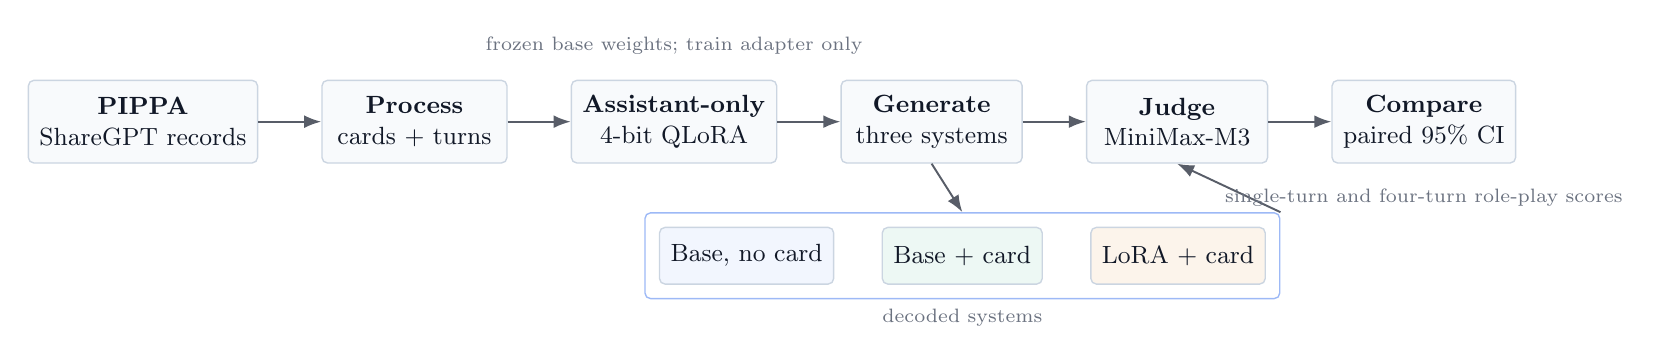
\begin{tikzpicture}[font=\small, node distance=6mm and 8mm]
    \node[paperBox, minimum width=2.25cm, minimum height=1.05cm] (raw)
      {\textbf{PIPPA}\\ShareGPT records};
    \node[paperBox, right=of raw, minimum width=2.35cm, minimum height=1.05cm] (process)
      {\textbf{Process}\\cards + turns};
    \node[paperBox, right=of process, minimum width=2.45cm, minimum height=1.05cm] (train)
      {\textbf{Assistant-only}\\4-bit QLoRA};
    \node[paperBox, right=of train, minimum width=2.30cm, minimum height=1.05cm] (generate)
      {\textbf{Generate}\\three systems};
    \node[paperBox, right=of generate, minimum width=2.30cm, minimum height=1.05cm] (judge)
      {\textbf{Judge}\\MiniMax-M3};
    \node[paperBox, right=of judge, minimum width=2.20cm, minimum height=1.05cm] (ci)
      {\textbf{Compare}\\paired 95\% CI};

    \draw[paperArrow] (raw) -- (process);
    \draw[paperArrow] (process) -- (train);
    \draw[paperArrow] (train) -- (generate);
    \draw[paperArrow] (generate) -- (judge);
    \draw[paperArrow] (judge) -- (ci);

    \node[paperBox, fill=paperBlue!6, below=8mm of generate, xshift=-2.35cm,
      minimum width=1.95cm, minimum height=0.72cm] (baseSys) {\base};
    \node[paperBox, fill=paperGreen!7, right=6mm of baseSys,
      minimum width=1.95cm, minimum height=0.72cm] (cardSys) {\card};
    \node[paperBox, fill=paperOrange!8, right=6mm of cardSys,
      minimum width=1.95cm, minimum height=0.72cm] (loraSys) {\lora};

    \node[draw=paperBlue!45, rounded corners=2pt, line width=0.5pt,
      fit=(baseSys)(cardSys)(loraSys), inner sep=5pt,
      label={[paperNote]below:decoded systems}] (systems) {};

    \draw[paperArrow] (generate.south) -- (systems.north);
    \draw[paperArrow] (systems.north east) -- (judge.south);

    \node[paperNote, above=2mm of train] {frozen base weights; train adapter only};
    \node[paperNote, below=2mm of ci] {single-turn and four-turn role-play scores};
  \end{tikzpicture}}
  \caption{Overall workflow. The same filtered evaluation prompts are decoded
  by \base, \card, and \lora, judged anonymously, and summarized with paired
  confidence intervals.}
  \label{fig:workflow}
\end{figure}%
}

\newcommand{\figLoraInjection}{%
\begin{figure}[H]
  \centering
  \resizebox{0.95\linewidth}{!}{%
  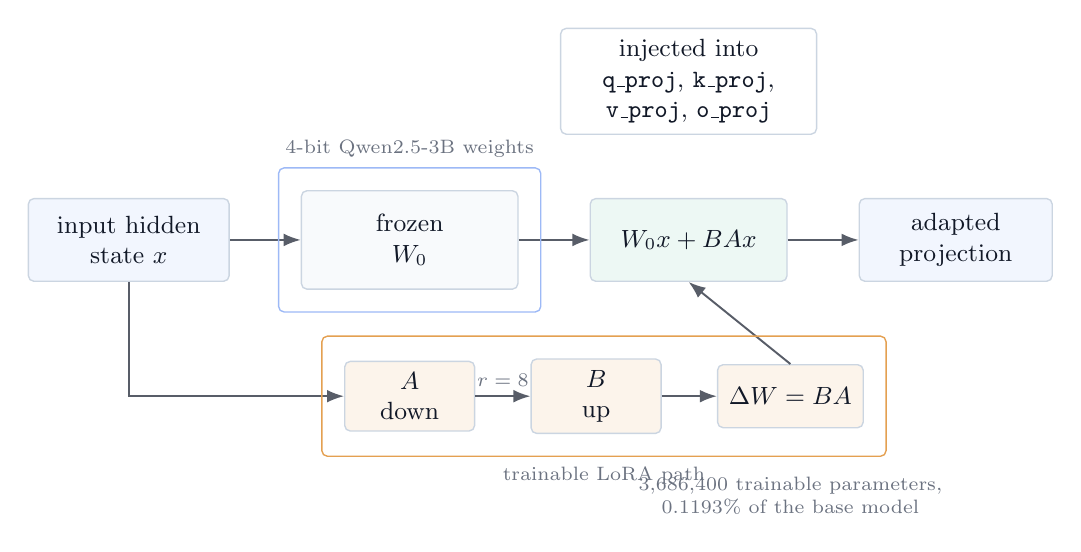
\begin{tikzpicture}[font=\small, node distance=8mm and 9mm]
    \node[paperBox, fill=paperBlue!6, minimum width=2.55cm,
      minimum height=1.05cm] (input) {input hidden\\state $x$};
    \node[paperBox, right=of input, fill=paperFill, minimum width=2.75cm,
      minimum height=1.25cm] (w0) {frozen\\$W_0$};
    \node[paperBox, right=of w0, fill=paperGreen!7, minimum width=2.50cm,
      minimum height=1.05cm] (sum) {$W_0x + BAx$};
    \node[paperBox, right=of sum, fill=paperBlue!6, minimum width=2.45cm,
      minimum height=1.05cm] (out) {adapted\\projection};

    \node[paperBox, below=9mm of w0, fill=paperOrange!8, minimum width=1.65cm,
      minimum height=0.80cm] (a) {$A$\\down};
    \node[paperBox, right=7mm of a, fill=paperOrange!8, minimum width=1.65cm,
      minimum height=0.80cm] (b) {$B$\\up};
    \node[paperBox, right=7mm of b, fill=paperOrange!8, minimum width=1.85cm,
      minimum height=0.80cm] (delta) {$\Delta W = BA$};

    \draw[paperArrow] (input) -- (w0);
    \draw[paperArrow] (w0) -- (sum);
    \draw[paperArrow] (sum) -- (out);
    \draw[paperArrow] (input.south) |- (a.west);
    \draw[paperArrow] (a) -- node[paperNote, above] {$r=8$} (b);
    \draw[paperArrow] (b) -- (delta);
    \draw[paperArrow] (delta.north) -- (sum.south);

    \node[draw=paperBlue!45, rounded corners=2pt, line width=0.5pt,
      fit=(w0), inner sep=8pt,
      label={[paperNote]above:4-bit Qwen2.5-3B weights}] {};
    \node[draw=paperOrange!70, rounded corners=2pt, line width=0.5pt,
      fit=(a)(b)(delta), inner sep=8pt,
      label={[paperNote]below:trainable LoRA path}] {};

    \node[paperBox, fill=white, above=8mm of sum, minimum width=3.25cm]
      {injected into\\\texttt{q\_proj}, \texttt{k\_proj},\\
      \texttt{v\_proj}, \texttt{o\_proj}};
    \node[paperNote, below=5mm of delta, text width=4.2cm]
      {3,686,400 trainable parameters, 0.1193\% of the base model};
  \end{tikzpicture}}
  \caption{LoRA injection schematic. The base attention projection is frozen,
  while a low-rank update path is trained for the selected Qwen2.5 attention
  projections.}
  \label{fig:lora-injection}
\end{figure}%
}

\newcommand{\figPairedEffects}{%
\begin{figure}[H]
  \centering
  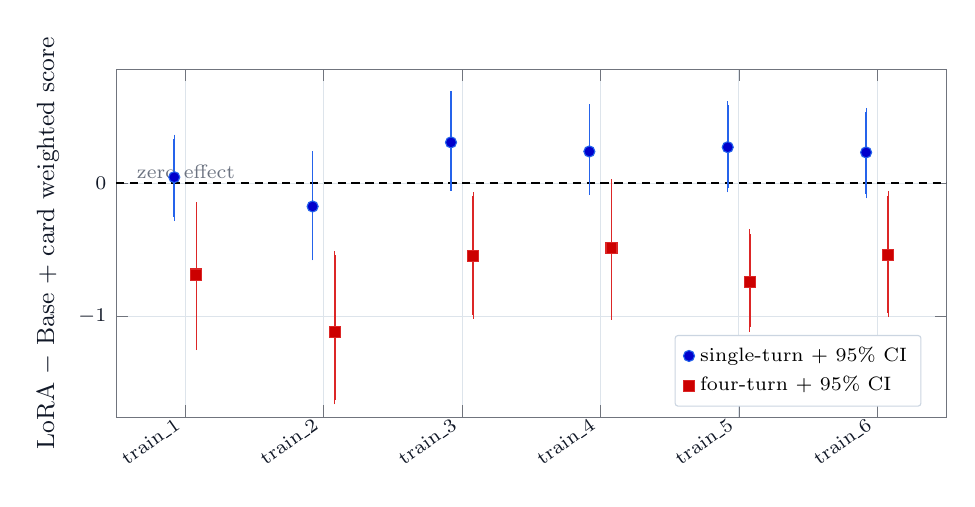
\begin{tikzpicture}
    \begin{axis}[
      paperAxis,
      height=6.0cm,
      xmin=0.5, xmax=6.5,
      ymin=-1.75, ymax=0.85,
      xtick={1,2,3,4,5,6},
      xticklabels={train\_1,train\_2,train\_3,train\_4,train\_5,train\_6},
      x tick label style={rotate=35, anchor=east, font=\scriptsize},
      ylabel={LoRA $-$ \card weighted score},
      legend pos=south east
    ]
      \addplot[black, densely dashed, line width=0.5pt, forget plot]
        coordinates {(0.5,0) (6.5,0)};
      \addplot+[
        only marks,
        mark=*,
        mark size=2.0pt,
        color=paperBlue,
        error bars/.cd,
        y dir=both,
        y explicit,
        error bar style={line width=0.6pt},
        error mark options={mark size=1.5pt}
      ] table[row sep=\\, x=x, y=y, y error plus=plus, y error minus=minus] {
        x y plus minus\\
        0.92 0.043 0.287 0.298\\
        1.92 -0.176 0.383 0.371\\
        2.92 0.303 0.353 0.332\\
        3.92 0.235 0.323 0.295\\
        4.92 0.267 0.313 0.306\\
        5.92 0.228 0.302 0.313\\
      };
      \addlegendentry{single-turn + 95\% CI}
      \addplot+[
        only marks,
        mark=square*,
        mark size=2.0pt,
        color=paperRed,
        error bars/.cd,
        y dir=both,
        y explicit,
        error bar style={line width=0.6pt},
        error mark options={mark size=1.5pt}
      ] table[row sep=\\, x=x, y=y, y error plus=plus, y error minus=minus] {
        x y plus minus\\
        1.08 -0.685 0.508 0.533\\
        2.08 -1.113 0.571 0.510\\
        3.08 -0.545 0.445 0.440\\
        4.08 -0.485 0.480 0.508\\
        5.08 -0.743 0.365 0.337\\
        6.08 -0.540 0.445 0.432\\
      };
      \addlegendentry{four-turn + 95\% CI}
      \node[anchor=west, font=\scriptsize, text=paperMuted]
        at (axis cs:0.58,0.08) {zero effect};
    \end{axis}
  \end{tikzpicture}
  \caption{Paired effects across six runs. Single-turn intervals cross zero,
  while all four-turn mean differences are negative against the prompted base
  model.}
  \label{fig:paired-effects}
\end{figure}%
}

\newcommand{\figRepetitionDiversity}{%
\begin{figure}[H]
  \centering
  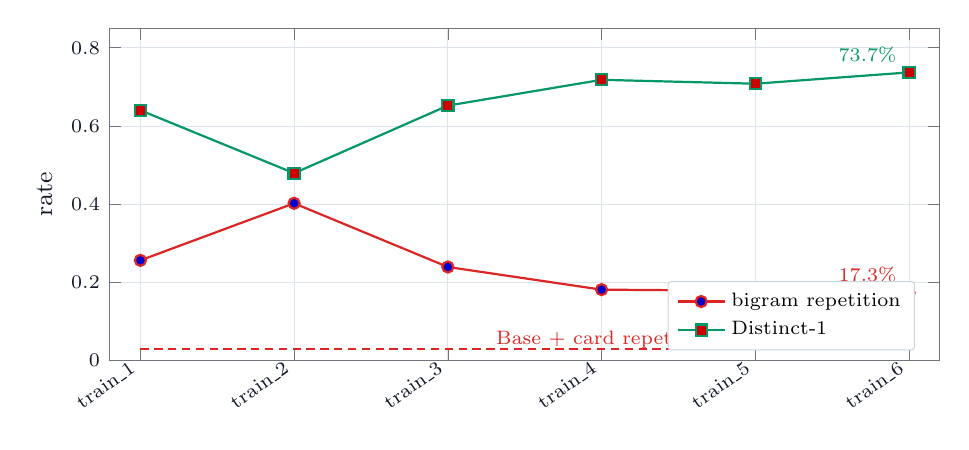
\begin{tikzpicture}
    \begin{axis}[
      paperAxis,
      height=5.8cm,
      xmin=0.8, xmax=6.2,
      ymin=0, ymax=0.85,
      xtick={1,2,3,4,5,6},
      xticklabels={train\_1,train\_2,train\_3,train\_4,train\_5,train\_6},
      x tick label style={rotate=35, anchor=east, font=\scriptsize},
      ylabel={rate},
      legend pos=south east
    ]
      \addplot+[
        color=paperRed,
        line width=0.8pt,
        mark=*,
        mark size=2.0pt
      ] coordinates {
        (1,0.256) (2,0.402) (3,0.239) (4,0.181) (5,0.178) (6,0.173)
      };
      \addlegendentry{bigram repetition}
      \addplot+[
        color=paperGreen,
        line width=0.8pt,
        mark=square*,
        mark size=2.0pt
      ] coordinates {
        (1,0.640) (2,0.479) (3,0.652) (4,0.718) (5,0.708) (6,0.737)
      };
      \addlegendentry{Distinct-1}
      \addplot[paperRed, densely dashed, line width=0.5pt, forget plot]
        coordinates {(1,0.029) (6,0.029)};
      \node[anchor=west, font=\scriptsize, text=paperRed]
        at (axis cs:3.25,0.055) {\card repetition 2.9\%};
      \node[anchor=south east, font=\scriptsize, text=paperRed]
        at (axis cs:5.98,0.173) {17.3\%};
      \node[anchor=south east, font=\scriptsize, text=paperGreen]
        at (axis cs:5.98,0.737) {73.7\%};
    \end{axis}
  \end{tikzpicture}
  \caption{Repetition and diversity trend. Later LoRA runs reduce repetition
  and recover Distinct-1, but train\_6 still has 17.3\% repetition, far above
  the 2.9\% \card baseline observed in train\_4.}
  \label{fig:repetition-diversity}
\end{figure}%
}


\begin{document}

\maketitle

\begin{abstract}
This project studies small-model role-play dialogue under limited computing
resources. Rather than proposing a new role-play method, we use controlled
comparisons to examine how persona prompting, QLoRA fine-tuning, data
formatting, and evaluation choices jointly affect role consistency and response
quality. We fine-tune Qwen2.5-3B-Instruct on PIPPA-ShareGPT role-play
conversations using 4-bit QLoRA and evaluate six training configurations
covering character-card-preserving truncation, longer context, lower learning
rate, data cleaning, and assistant-turn window training. Each evaluation
compares three systems: the base model without a character card, the base model
with a character card, and the LoRA-adapted model with the same card. Automatic
metrics are combined with anonymous MiniMax-M3 judging for single-turn and
four-turn dialogue. The results show that QLoRA can learn the target response
distribution and reduce some generic assistant behavior; the best LoRA variants
reach a 55.6\% single-turn win rate against the prompted base model, and
repetition decreases from 40.2\% in an early run to 17.3\% in the final
window-based run. However, all single-turn paired confidence intervals include
zero, and all completed LoRA systems remain weaker than the prompted base model
in multi-turn evaluation. These findings suggest that role-play improvement in
small models cannot be attributed to parameter adaptation alone, and still
depends on data quality, context modeling, and evaluation reliability.
\end{abstract}

\section{Introduction}

Large language models have achieved strong performance in open-domain dialogue,
instruction following, and general text generation. However, role-play dialogue
generation remains a challenging setting. Unlike general conversational tasks,
role-play requires a model not only to produce relevant and natural responses,
but also to consistently maintain a target character's persona, tone, values,
and narrative perspective across multiple turns. For this type of application,
users often care not only about whether a response is reasonable, but also
whether it sounds like something the character would actually say.

A common approach to role-play is prompt-based persona conditioning, where a
character card or persona description is provided in the system prompt. This
approach is simple to implement, relatively inexpensive to deploy, and often
effective in eliciting character-like responses. However, prompt-based methods
alone are often insufficient for stable role-play. Models may fall back to
generic assistant-style language, produce meta discourse, or drift away from
the intended persona. In multi-turn interactions, they may also show identity
inconsistency, weak memory continuity, or repetitive generation. In other
words, prompting can activate role-play behavior, but it does not necessarily
sustain it reliably.

In this context, parameter-efficient fine-tuning offers a practical direction
for role-play adaptation. Compared with full fine-tuning, LoRA and its
quantized variant QLoRA enable task adaptation with substantially lower
computational and memory cost, making them suitable for small-model
customization under limited resources. This leads to a natural question: when a
base model already exhibits some role-play ability with the help of a character
card, can LoRA fine-tuning further improve role expression and consistency? If
so, where does the improvement mainly appear? If not, are the main limitations
caused by parameter adaptation itself, or by other factors such as data
quality, context modeling, and evaluation design?

Answering this question is not simply a matter of training a LoRA model for
role-play. In practice, the final quality of a role-play system is jointly
affected by prompt design, training data format, supervision strategy, and
evaluation settings. These factors are often intertwined, making the actual
contribution of fine-tuning difficult to isolate. For this reason, it is useful
to examine role-play adaptation under controlled comparisons, so that the
effects of persona prompting and parameter-efficient fine-tuning can be
observed more clearly.

Motivated by this consideration, we conduct LoRA-based role-play experiments on
Qwen2.5-3B-Instruct using character dialogue data under a resource-constrained
setting. We compare several configurations under matched evaluation conditions.
For evaluation, we combine automatic metrics with LLM-as-Judge assessment
\citep{zheng2023judging}, and examine model behavior from several aspects,
including role adherence,
multi-turn consistency, repetition, and refusal tendency.

This work does not aim to propose a new role-play method. Instead, through
controlled comparative experiments, we study how prompt conditioning,
parameter-efficient fine-tuning, data format, and evaluation choices jointly
affect role-play performance in practice, and we summarize several empirical
observations from the results. Our experiments suggest that LoRA fine-tuning
shows a single-turn improvement trend and can reduce generic assistant-style
responses in some settings, but its advantage over a strong \card baseline is
not yet consistently significant, and its multi-turn performance still remains
weaker overall. These findings indicate that improving small-model role-play
quality cannot be attributed to parameter adaptation alone, but depends on the
joint effect of data quality, context modeling, and evaluation design.

The remainder of this paper is organized as follows. Section~2 reviews the
role-play dialogue setting, the limitations of prompt-based persona
conditioning, and the motivation for using LoRA/QLoRA under limited resources.
Section~3 presents our method, including the training pipeline, data processing,
truncation strategy, and evaluation design. Section~4 describes the
experimental setup and the six completed training variants. Section~5 reports
the main results from automatic metrics, paired comparisons, and LLM-as-Judge
evaluation. Section~6 discusses the main findings and their implications.
Section~7 then integrates the limitations of the current study with the final
conclusion, so that the closing argument remains compact and directly tied to
the evidence. The project repository is available at
\url{https://github.com/yeunmer2006/26ML-roleplay-lora.git}.

\section{Background}

\subsection{Role-Play Dialogue Generation}

Role-play dialogue generation is a conditional generation task centered on a
predefined character. Compared with general instruction-following tasks, it
requires the model not only to produce responses relevant to user input, but
also to consistently reflect the target persona in wording, tone, values, and
narrative perspective. In multi-turn settings, the model is further expected to
maintain relatively stable character identity and memory continuity as the
dialogue develops.

The difficulty of this task mainly lies in three aspects. First, character
information is usually provided in the form of a character card or persona
description, and the model needs to translate these descriptions into stable
generation behavior. Second, multi-turn dialogue continuously introduces new
context, so persona information, dialogue history, and current user input may
compete with one another, especially under limited context windows. Third,
role-play quality is inherently open-ended: a single reference answer is often
insufficient to determine whether a response truly sounds like the target
character, which makes standard reference-based metrics less adequate for
evaluation.

\subsection{Limitations of Prompt-Based Persona Conditioning}

A common approach is to control the base model through a persona prompt or
character card. This method does not require additional training, has
relatively low deployment cost, and can often produce noticeable improvements
in short role-play conversations.

However, this approach also has limitations. Base models are typically biased
toward general assistant behavior, and their default safety language,
explanatory style, and neutral phrasing may conflict with role-play objectives.
At the same time, prompts operate only at inference time and do not change the
model's underlying task preference, so their effect may weaken as the context
becomes longer. When the target persona has a strong speaking style or the
multi-turn setting becomes more complex, prompting alone is often insufficient
to maintain stable role consistency.

\subsection{LoRA and QLoRA}

LoRA is a commonly used parameter-efficient fine-tuning method. It freezes most
pretrained parameters and introduces low-rank update matrices into selected
linear layers, allowing task adaptation with relatively low training cost
\citep{hu2022lora}. Given a pretrained matrix $W_0$, LoRA computes
\begin{equation}
  W = W_0 + \Delta W = W_0 + BA,
\end{equation}
where the rank of $BA$ is much smaller than the dimensions of $W_0$. Under
limited computational resources, this offers a practical balance between
efficiency and experimental flexibility.

QLoRA further combines LoRA with low-bit quantization by loading the base model
in 4-bit form while keeping LoRA parameters trainable, which substantially
reduces memory usage \citep{dettmers2023qlora}. For the Qwen2.5-3B-Instruct
model used in this work, QLoRA makes multiple role-play fine-tuning experiments
feasible on consumer-grade GPUs.

Still, the trainability of LoRA does not directly imply improved role-play
quality. For this task, the more relevant question is whether fine-tuning
actually improves role expression, consistency, and common failure patterns,
rather than merely reducing training loss.

\subsection{Problem Setting of This Work}

This work focuses on a specific question: when a character card is already
provided as a strong conditioning signal, can parameter-efficient fine-tuning
further improve role-play performance in small models? In this study, LoRA is
treated as a testable adaptation method rather than a guaranteed solution. The
following method and experiments are designed to examine its practical effect
on role expression, multi-turn consistency, and common failure patterns.

\section{Method}

\figWorkflow

Figure~\ref{fig:workflow} summarizes the controlled pipeline used throughout
the study. The workflow starts from PIPPA-ShareGPT records, converts character
profiles and dialogue turns into supervised role-play examples, and trains only
the QLoRA adapter while keeping the base model frozen. At evaluation time, the
same filtered prompts are decoded by all three systems: \base isolates the
unconditioned base-model behavior, \card measures the effect of prompt-time
persona conditioning, and \lora measures the additional effect of the trained
adapter under the same character card. The anonymous MiniMax-M3 judge then
scores matched outputs without seeing system identities. Finally, paired
bootstrap confidence intervals are used to compare systems on the same
single-turn and four-turn samples.

\subsection{Base Model and Adapter}

The base model is Qwen2.5-3B-Instruct \citep{qwen2024qwen25}. We load it with
4-bit NF4 quantization, double quantization, and FP16 computation. During
training, the base weights are frozen and LoRA adapters are inserted into the
attention projection layers: \texttt{q\_proj}, \texttt{k\_proj},
\texttt{v\_proj}, and \texttt{o\_proj}. All experiments use rank $r=8$,
LoRA alpha 16, dropout 0.05, and no bias update. This trains 3,686,400
parameters, approximately 0.1193\% of the 3.09B-parameter base model.

\figLoraInjection

Figure~\ref{fig:lora-injection} illustrates the adapter mechanism used in all
training runs. For each selected attention projection, the quantized base
matrix $W_0$ remains frozen, so the original projection path still computes
$W_0x$ from the input hidden state. In parallel, the trainable LoRA path maps
the same hidden state through a rank-$8$ down projection $A$ and an up
projection $B$, producing the additive update $BAx$. The adapted projection is
therefore $W_0x + BAx$, which changes the model's response distribution without
updating the base weights themselves. We inject this low-rank path into
\texttt{q\_proj}, \texttt{k\_proj}, \texttt{v\_proj}, and \texttt{o\_proj},
leaving only 3,686,400 parameters trainable, or 0.1193\% of the base model.

\subsection{Data Processing}

We use the PIPPA-ShareGPT-formatted dataset
\citep{gosling2023pippa,karakarawitch2023pippa}. Each record contains a
character profile and a
multi-turn conversation. The processing pipeline removes invalid samples,
maps human messages to the user role and model messages to the assistant role,
and builds the system prompt from the character name and description:
\begin{quote}
  \texttt{Character name: <name>}\\
  \texttt{<description>}
\end{quote}
The current processed snapshot contains 9,211 training, 1,152 validation, and
1,152 test conversations. Most formal runs sample at most 4,000 training
examples and 200 validation examples with seed 42. The exception is train\_6:
its configuration sets \texttt{max\_train\_samples=2500} and
\texttt{max\_eval\_samples=120}, then assistant-window expansion produces
5,198 training windows and 261 validation windows. Because the six archived
runs used multiple data snapshots, cross-experiment differences are interpreted
as trends rather than strict single-variable causal effects.

\subsection{Assistant-Only Supervision}

The full conversation is rendered with the model's chat template, but loss is
computed only on assistant tokens. System, user, and padding tokens are assigned
label \texttt{-100}. This objective teaches the model to generate role
responses rather than reproduce the character card or user input.

\subsection{Truncation and Windowing}

The initial implementation used token-level left truncation. This could remove
the character card before the supervised response, weakening persona
conditioning during training. We therefore add a message-level truncation
strategy that always keeps the complete system character card, removes
unsupervised messages after the final assistant response, and drops the oldest
dialogue messages first. Training and assistant perplexity evaluation reuse the
same truncation logic.

The final experiment adds an \texttt{assistant\_windows} strategy. Instead of
creating one training sample from the latest conversation suffix, it creates up
to three target assistant-turn windows from a conversation. Each window keeps
the character card and the nearest preceding context, but supervises only the
target assistant response. This tests whether training on more next-turn
contexts improves multi-turn role-play behavior.

\section{Experimental Setup}

\subsection{Training Configurations}

Table~\ref{tab:training-configs} summarizes the six completed experiments. All
runs use batch size 1, gradient accumulation 8, the \texttt{paged\_adamw\_8bit}
optimizer, cosine scheduling, weight decay 0.01, and gradient checkpointing.

\begin{table}[t]
  \centering
  \caption{Training configurations. Snapshot labels indicate that archived
  runs did not all use the same processed data files.}
  \label{tab:training-configs}
  \small
  \begin{tabular}{llrrrll}
    \toprule
    Run & Main change & Context & LR & Epochs & Steps & Snapshot \\
    \midrule
    train\_1 & Old left truncation & 512 & 2e-4 & 1 & 500 & A \\
    train\_2 & Preserve character card & 512 & 2e-4 & 1 & 500 & B \\
    train\_3 & Longer context & 1024 & 2e-4 & 1 & 500 & C \\
    train\_4 & Lower LR, best checkpoint & 1024 & 1e-4 & 2 & 1000 & A \\
    train\_5 & Clean-data run manifest & 1024 & 1e-4 & 2 & 942 & C manifest \\
    train\_6 & Assistant-turn windows & 1024 & 1e-4 & 1 & 650 & D \\
    \bottomrule
  \end{tabular}
\end{table}

\subsection{Evaluation Protocol}

Each run evaluates three systems:
\begin{itemize}
  \item \base: the base model without character-card conditioning;
  \item \card: the base model with the character card as the system prompt;
  \item \lora: the LoRA-adapted model with the same character card.
\end{itemize}
The main comparison is \lora against \card. The comparison between \card and
\base estimates the contribution of prompting alone.

The evaluator filters unsafe or low-quality test records, uses stable hash
ordering with seed 42, keeps at most one sample per character, and selects up
to 100 single-turn samples plus 20 four-turn challenges. Generation uses greedy
decoding with at most 256 new tokens. Automatic metrics include assistant
reference perplexity, Distinct-1/2, bigram repetition rate, empty-or-refusal
rate, throughput, and GPU memory.

MiniMax-M3 is used as an anonymous judge, following the LLM-as-Judge evaluation
paradigm \citep{zheng2023judging}. Single-turn scoring uses five dimensions:
role identity, style, relevance, naturalness, and immersion. Their weights are
35\%, 20\%, 20\%, 15\%, and 10\%. Multi-turn scoring uses role identity,
memory, coherence, style, and immersion, with weights 25\%, 25\%, 20\%, 15\%,
and 15\%. We report paired differences, win rates, judge success rates, order
consistency checks, and 1,000-sample bootstrap 95\% confidence intervals.

\section{Results}

\subsection{Character Cards Are a Strong Baseline}

Table~\ref{tab:train4-systems} shows the three-system comparison from
train\_4. Adding the character card to the base model improves the single-turn
weighted score from 1.938 to 2.703, a gain of 0.765. It also improves the
multi-turn weighted score from 1.882 to 3.153, a gain of 1.270. These gains are
larger than the additional single-turn gain produced by the LoRA adapter in the
same run.

\begin{table}[t]
  \centering
  \caption{Three-system comparison in train\_4. This run has high judge order
  consistency and is the clearest example of the role-card prompting baseline.}
  \label{tab:train4-systems}
  \small
  \begin{tabular}{lrrrrr}
    \toprule
    System & PPL $\downarrow$ & Repetition $\downarrow$ & Refusal $\downarrow$ &
    Single $\uparrow$ & Multi $\uparrow$ \\
    \midrule
    \base & 872.614 & 0.027 & 0.090 & 1.938 & 1.882 \\
    \card & 94.725 & 0.029 & 0.040 & 2.703 & 3.153 \\
    \lora & 10.343 & 0.181 & 0.010 & 2.938 & 2.668 \\
    \bottomrule
  \end{tabular}
\end{table}

\subsection{LoRA Learns the Role-Play Response Distribution}

Across all six runs, the \lora system obtains assistant reference perplexity
between 9.441 and 11.096, while the \card baseline in train\_4 has PPL 94.725.
This suggests that QLoRA substantially changes the model's probability
distribution toward the supervised role-play responses. However, this
adaptation does not directly imply better role-play quality. Train\_2 has the
lowest PPL, 9.441, but also the highest repetition rate, 40.2\%, and the
lowest multi-turn score, 2.225.

\begin{table}[t]
  \centering
  \caption{Core \lora results across six experiments. Single-turn sample counts
  are 70 for train\_2, 99 for train\_3/train\_4, and 100 for the other runs.}
  \label{tab:lora-results}
  \small
  \begin{tabular}{lrrrrrr}
    \toprule
    Run & PPL $\downarrow$ & Identity $\uparrow$ & Single $\uparrow$ &
    Win vs. \card & Repetition $\downarrow$ & Multi $\uparrow$ \\
    \midrule
    train\_1 & 10.404 & 2.770 & 2.718 & 44.0\% & 25.6\% & 2.763 \\
    train\_2 & 9.441 & 2.657 & 2.643 & 48.6\% & 40.2\% & 2.225 \\
    train\_3 & 10.446 & 2.970 & 2.935 & 55.6\% & 23.9\% & 2.890 \\
    train\_4 & 10.343 & 2.909 & 2.938 & 55.6\% & 18.1\% & 2.668 \\
    train\_5 & 10.760 & 2.950 & 2.989 & 55.0\% & 17.8\% & 2.780 \\
    train\_6 & 11.096 & 2.820 & 2.921 & 50.0\% & 17.3\% & 2.780 \\
    \bottomrule
  \end{tabular}
\end{table}

\subsection{Single-Turn Improvement Is a Trend, Not a Conclusive Win}

Train\_3, train\_4, and train\_5 show the strongest single-turn role-play
results. Train\_3 and train\_4 reach a 55.6\% win rate against \card, and
train\_5 obtains the highest single-turn weighted score, 2.989. Qualitatively,
the adapter can reduce generic assistant behavior. For example, in train\_4,
the prompted base model sometimes explains that a threatening role-play scene
is fictional, while the LoRA model responds directly in character.

Nevertheless, Table~\ref{tab:paired} shows that the single-turn paired
confidence intervals all include zero. The evidence supports an improvement
trend, but not a statistically stable advantage over the prompted base model.

\figPairedEffects

Figure~\ref{fig:paired-effects} visualizes the paired mean difference
\lora$-\card$ for each completed run. Each point compares the two systems on
the same evaluation samples, and each error bar shows the paired 95\%
confidence interval estimated by bootstrap resampling. Blue circular markers
show single-turn effects, while red square markers show four-turn effects. The
dashed zero line represents no advantage for either system: points above it
favor \lora, and points below it favor \card. Most single-turn means are
positive but their intervals cross zero, whereas all four-turn means are
negative, matching the conclusion that the adapter trend does not yet become a
stable multi-turn improvement.

\begin{table}[t]
  \centering
  \caption{Paired \lora minus \card differences. Positive values favor LoRA.
  All single-turn intervals include zero, while all multi-turn intervals are
  below or nearly below zero.}
  \label{tab:paired}
  \small
  \begin{tabular}{lrrr}
    \toprule
    Run & Single diff & Single 95\% CI & Multi diff / 95\% CI \\
    \midrule
    train\_1 & +0.043 & [-0.255, 0.330] & -0.685 / [-1.218, -0.177] \\
    train\_2 & -0.176 & [-0.547, 0.207] & -1.113 / [-1.623, -0.542] \\
    train\_3 & +0.303 & [-0.029, 0.656] & -0.545 / [-0.985, -0.100] \\
    train\_4 & +0.235 & [-0.060, 0.558] & -0.485 / [-0.993, -0.005] \\
    train\_5 & +0.267 & [-0.039, 0.580] & -0.743 / [-1.080, -0.378] \\
    train\_6 & +0.228 & [-0.085, 0.530] & -0.540 / [-0.972, -0.095] \\
    \bottomrule
  \end{tabular}
\end{table}

\subsection{Multi-Turn Role-Play Remains Worse Than Prompting}

The strongest negative result is multi-turn evaluation. All six LoRA variants
underperform \card in the four-turn challenge. In train\_4, the \card system
scores 3.153, while \lora scores 2.668. The paired difference is -0.485 with a
95\% confidence interval of [-0.993, -0.005]. Train\_6, which explicitly uses
assistant-turn windows, improves the memory dimension slightly compared with
train\_5, from 3.600 to 3.700, but the overall multi-turn score remains 2.780
and its win rate against \card decreases from 25.0\% to 20.0\%.

This suggests that supervised adapter training on next-response data does not
automatically teach stable long-context role maintenance. The model can fit
assistant responses and still lose identity, coherence, style, or immersion as
the conversation progresses.

\subsection{Repetition Is Reduced but Still a Major Gap}

Optimization and data changes reduce repetition. Train\_2 has a repetition
rate of 40.2\%. Increasing context length reduces it to 23.9\% in train\_3.
Lowering the learning rate and using the best checkpoint reduces it further to
18.1\% in train\_4. Data cleaning and assistant-window training reach 17.8\%
and 17.3\% in train\_5 and train\_6.

\figRepetitionDiversity

Figure~\ref{fig:repetition-diversity} tracks the main automatic quality gap
across LoRA runs. The red curve reports bigram repetition, while the green
curve reports Distinct-1 as a simple lexical diversity measure. Later training
choices reduce repetition from the early peak and recover diversity, so the
final assistant-window run reaches 17.3\% repetition and 73.7\% Distinct-1.
This trend suggests that context length, checkpoint choice, data cleaning, and
windowed supervision help suppress some loop-like outputs. However, the dashed
\card reference remains much lower at 2.9\% repetition, so repetition is still
the clearest remaining quality gap between the best LoRA system and prompting
alone.

Representative failures behind this gap include repeated promises, repeated
action templates, and loop-like phrasing.

\section{Discussion}

\paragraph{Prompting and fine-tuning play different roles.}
The character card is a strong inference-time conditioning signal. It improves
both single-turn and multi-turn scores before any parameter update. QLoRA then
pushes the model distribution closer to role-play reference responses, which is
visible in PPL and some single-turn judge dimensions. The two effects are not
equivalent: prompting preserves explicit persona information at inference time,
while LoRA changes response tendencies learned from the dataset.

\paragraph{Longer context appears helpful but is not isolated.}
Moving from 512 to 1024 context correlates with better single-turn role
identity and lower repetition when comparing train\_2 and train\_3. However,
the archived runs use different data hashes and different effective judge
sample counts. We therefore describe this as a trend rather than a causal
ablation result.

\paragraph{Low loss is not enough.}
Train\_2 has the lowest PPL but the worst repetition and lowest multi-turn
score. Train\_6 has the best validation loss among later runs but does not
improve multi-turn weighted score over train\_5. These observations suggest
that language-modeling objectives and reference PPL are useful for checking
whether training occurred, but they are insufficient as final role-play
metrics.

\section{Limitations and Conclusion}

This study shows that QLoRA makes role-play adaptation of
Qwen2.5-3B-Instruct practical on limited hardware, and the resulting LoRA
models do learn the target dialogue distribution: assistant-style refusals
decrease, single-turn judge scores show an overall improvement trend, and later
configurations reduce repetition relative to earlier LoRA runs. However, the
evidence does not support a stronger claim that LoRA has already established a
stable advantage over a strong \card baseline. Across the current paired
comparisons, single-turn confidence intervals still include zero, and all
completed LoRA systems remain weaker than \card on multi-turn overall quality.

These results should be interpreted together with several limitations. The six
training runs were not all produced from one frozen data snapshot, so some
comparisons are informative but not fully single-variable. The present split
also still needs a stricter audit for character overlap across train and test
partitions. On the evaluation side, the judge pipeline currently depends on one
model, a limited sample size, and a forced-choice setup without ties; in
addition, the multi-turn benchmark covers only a small set of four-turn Chinese
prompts. For this reason, the current results are best read as controlled
empirical evidence about trends and failure modes, rather than as a final
ranking of methods.

Taken together, the main conclusion of this work is that prompt conditioning
and parameter-efficient fine-tuning play different roles in small-model
role-play. A well-written character card already provides a strong baseline,
while LoRA mainly offers a possible single-turn style gain and some reduction
of generic assistant behavior. The remaining bottlenecks are multi-turn
identity maintenance, repetition control, and evaluation reliability. The next
stage should therefore prioritize a fixed and audited data snapshot, stricter
single-variable ablations, improved multi-turn training targets or preference
optimization, and a more robust evaluation protocol with blinded human review
or multiple judges.

\bibliographystyle{plainnat}
\bibliography{references}

\end{document}
